\documentclass[letterpaper,12pt]{article}

% things needed to include figures
\usepackage{subfigure, graphicx}
% float must be included for the [H] to actually work
\usepackage{float}
% formulas
\usepackage{amsmath}
% Added to adjust captions
\usepackage[singlelinecheck=false]{caption}
% added to adjust margins at the suggestion of Dr. Matt
\usepackage[top=1in, bottom=1in, left=1in, right=1in]{geometry}
\usepackage{fullpage}
\title{Photon Statistics}
\author{Max Bigras and David Frawley}

\begin{document}

\maketitle

\begin{abstract}
We explored the statistics for photons arriving from a constant intensity and a randomly scattered light source. We measured the number of photons arriving per a unit time. By constructing probability distributions and calculating $\chi^{2}$ values we found the distribution for constant intensity light to agree with a Poisson distribution and the distribution for randomly scattered light to agree with a Bose-Einstein distribution.
\end{abstract}

\section{Introduction}
We used a photomultiplier tube (PMT) and a photon counter to directly count the number of photons arriving per a unit time from two different light sources. By overlaying our experimental distribution over a theoretical distribution based on statistics we illustrated the probabilistic nature of the photodetection process itself \cite{koc}.



\section{Theory}
The probability for ejection of an electron from the PMT photocathode depends only on intensity light \cite{manual}. We are interested in the probability for obtaining $n$ counts in some large time interval $T$, for a constant intensity light source and a randomly scattered light source. 

For a constant intensity light source and from statistics the probability of detecting $n$ photons in time $T$ is

\begin{equation}
P(n,T) = \frac{n_{\mathrm{av}}^{n}}{n!}e^{-n_{\mathrm{av}}}
\label{poisson}
\end{equation}
where $n_{\mathrm{av}}$ is the average number of photons counted in time $T$.

But this is the Poisson distribution. So we expect a constant intensity light source to cause electrons to be ejected from the cathod of the PMT with a Poisson distribution.

What if the intensity of light varies in space randomly? This is the case for randomly scattered light. If one can determine the intensity of the light at any spatial location,  and perform a weighted average then the probability for detecting $n$ photons in time $T$ is

\begin{equation}
P(n,T) = \frac{n_{\mathrm{av}}^{n}}{(n_{\mathrm{av}}+1)^{n+1}}
\label{bose}
\end{equation}

But this is the Bose-Einstein distribution. So we expect a randomly scattered light source to cause electrons to be ejected from the cathod of the PMT with a Bose-Einstein distribution.

\section{Apparatus}
Our apparatus is shown in Figure \ref{apparatus}. We used photons produced by an HeNe laser, which emits around $10^{18}$ photons per a second. We are interested in counting a few thousand photons per a second, so we are required to reduce the intensity of the laser. We attenuate the laser in three ways, first we polarize the laser beam, then we spread it out with a short focal length lens and finally we pass the light through two pinholes ($<$100 $\mu$m diameter). Any surviving photons are detected by the the PMT and finally counted by the photon counter. The photon counter detects pulses above a discriminator level and counts the number of pulses per a unit time.
\begin{figure}[H]
  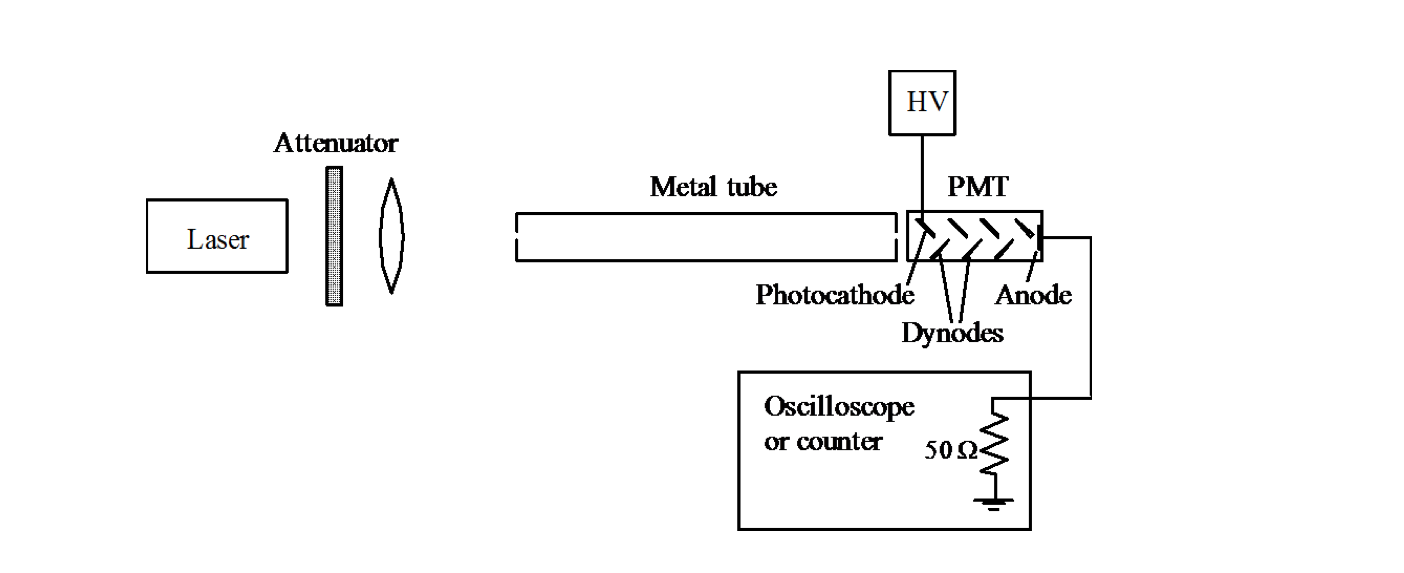
\includegraphics[totalheight=0.5\textwidth]{figs/apparatus}
  \caption{Diagram for apparatus}
  \label{apparatus}
\end{figure}

It's important to count pulses coming from photons and not from noise in the PMT. We measured how the count rate varies with increasing discriminator level. Initially there is a fast change as the noise gets filtered out, shown in Figure \ref{dlevel}, then the curve flattens out and again dips down as we began to also filter out the pulses from the photons. Because we're interested in detecting photons away from the noise we chose our discriminator level to be in the flat region.
\begin{figure}[H]
  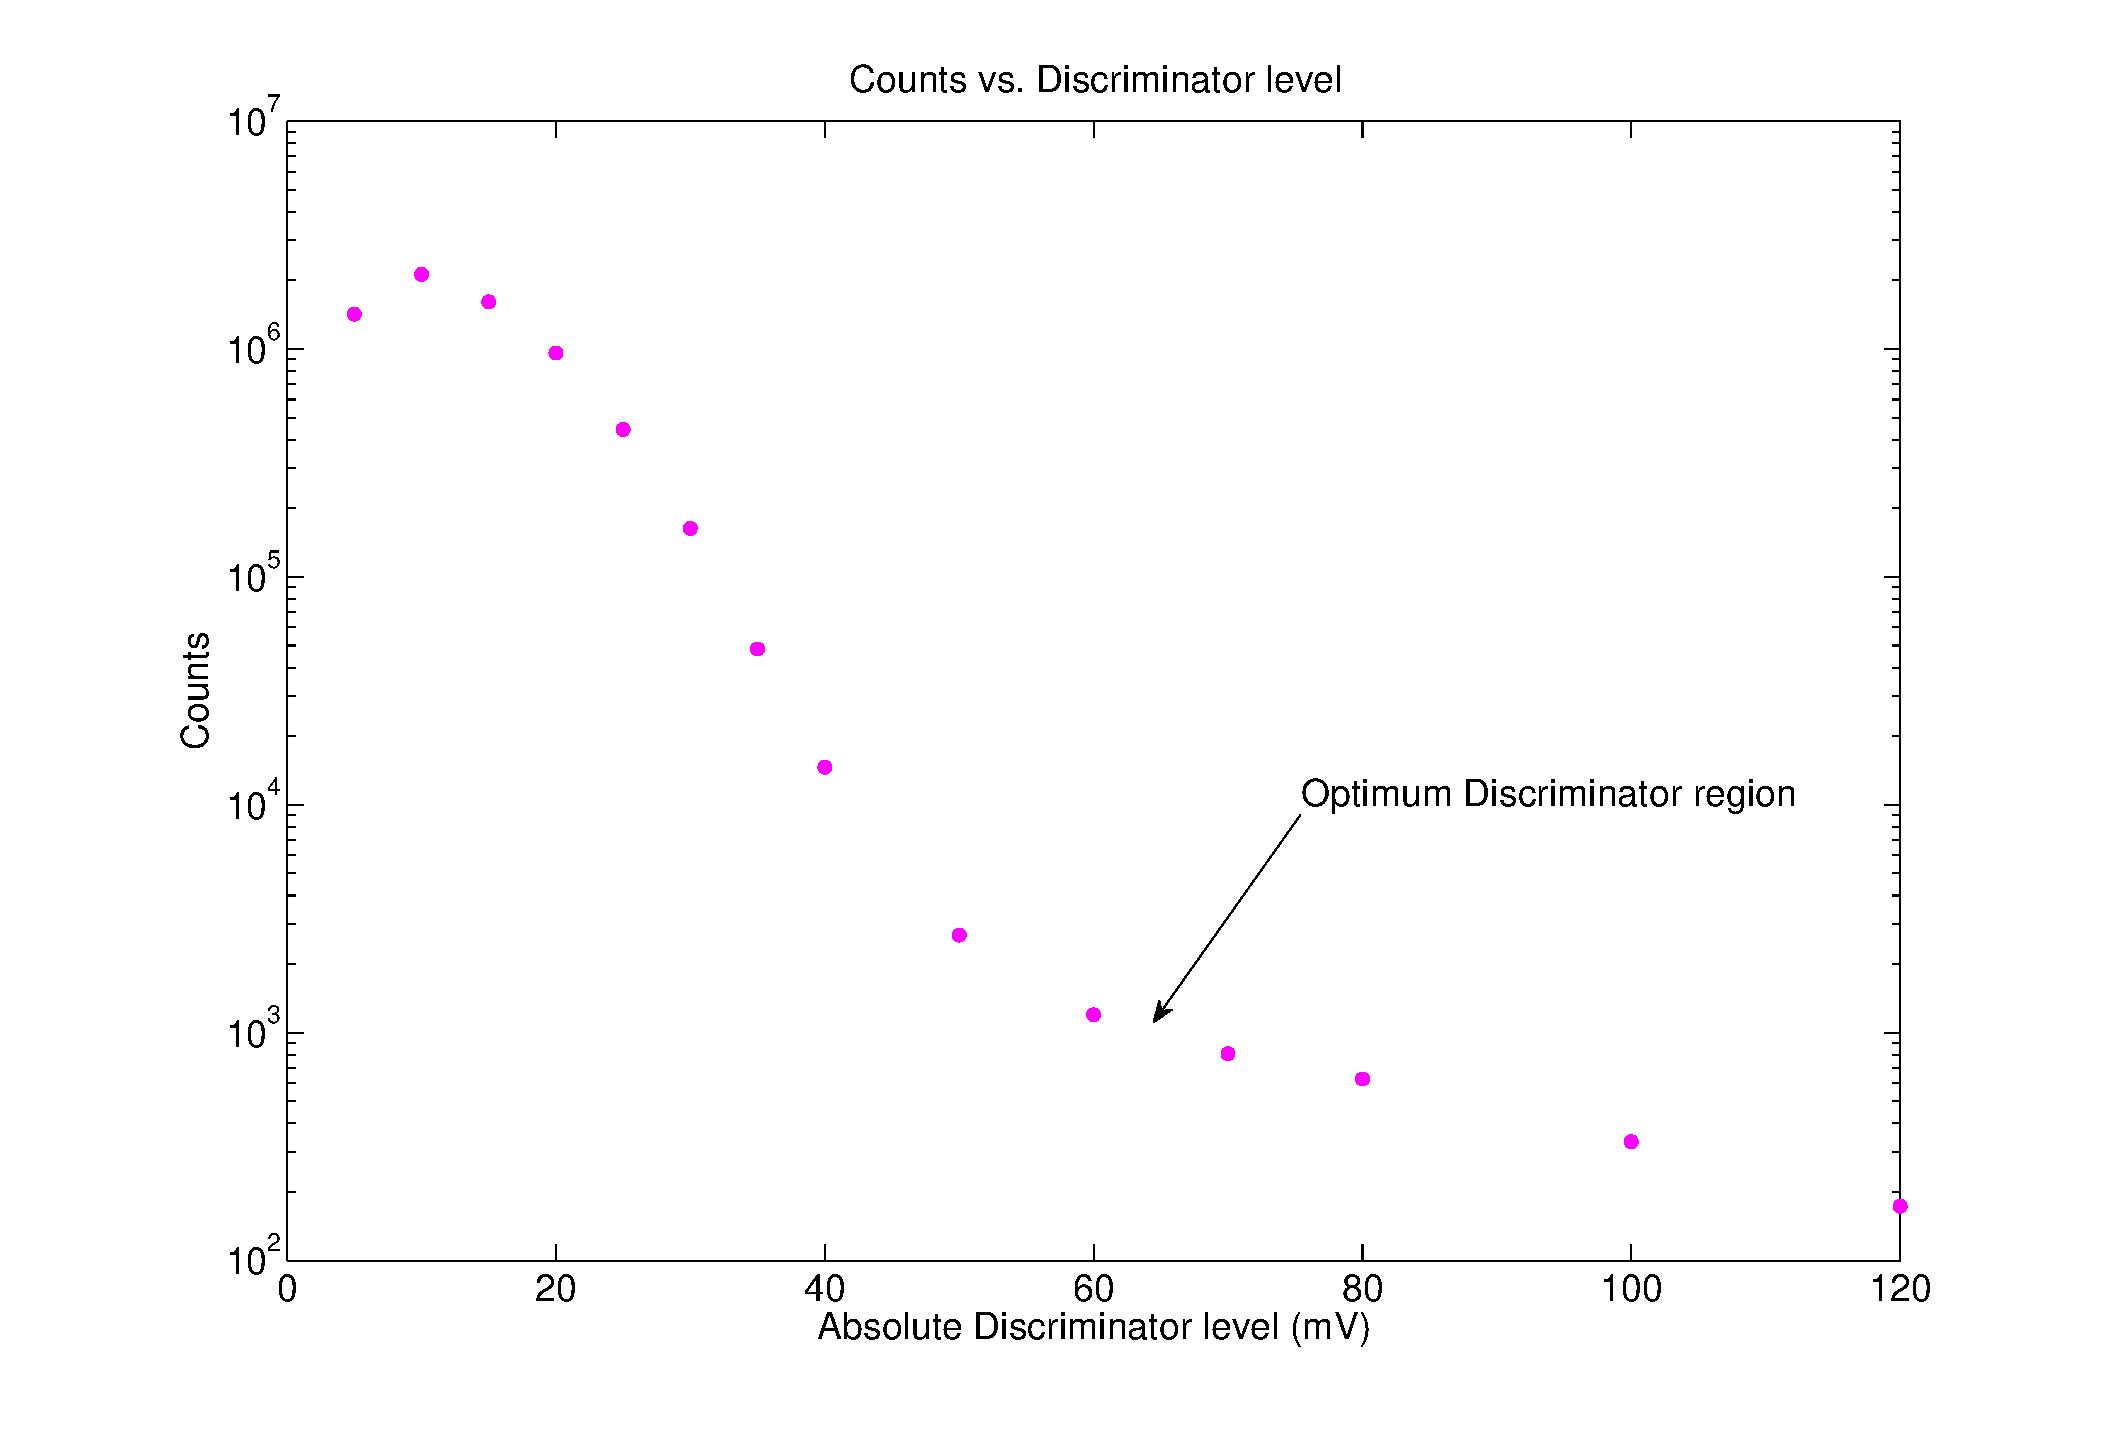
\includegraphics[totalheight=0.6\textwidth]{figs/dlevel}
  \caption{Finding the optimum discriminator level}
  \label{dlevel}
\end{figure}

\section{Analysis}
Figures \ref{ci1000}, \ref{ci3000} and \ref{ci10000} show our probability distributions for constant intensity light. As shown by the $\chi^{2}$ values and visually our experimental distributions agree with the theoretical Poisson distribution.
\begin{figure}[H]
  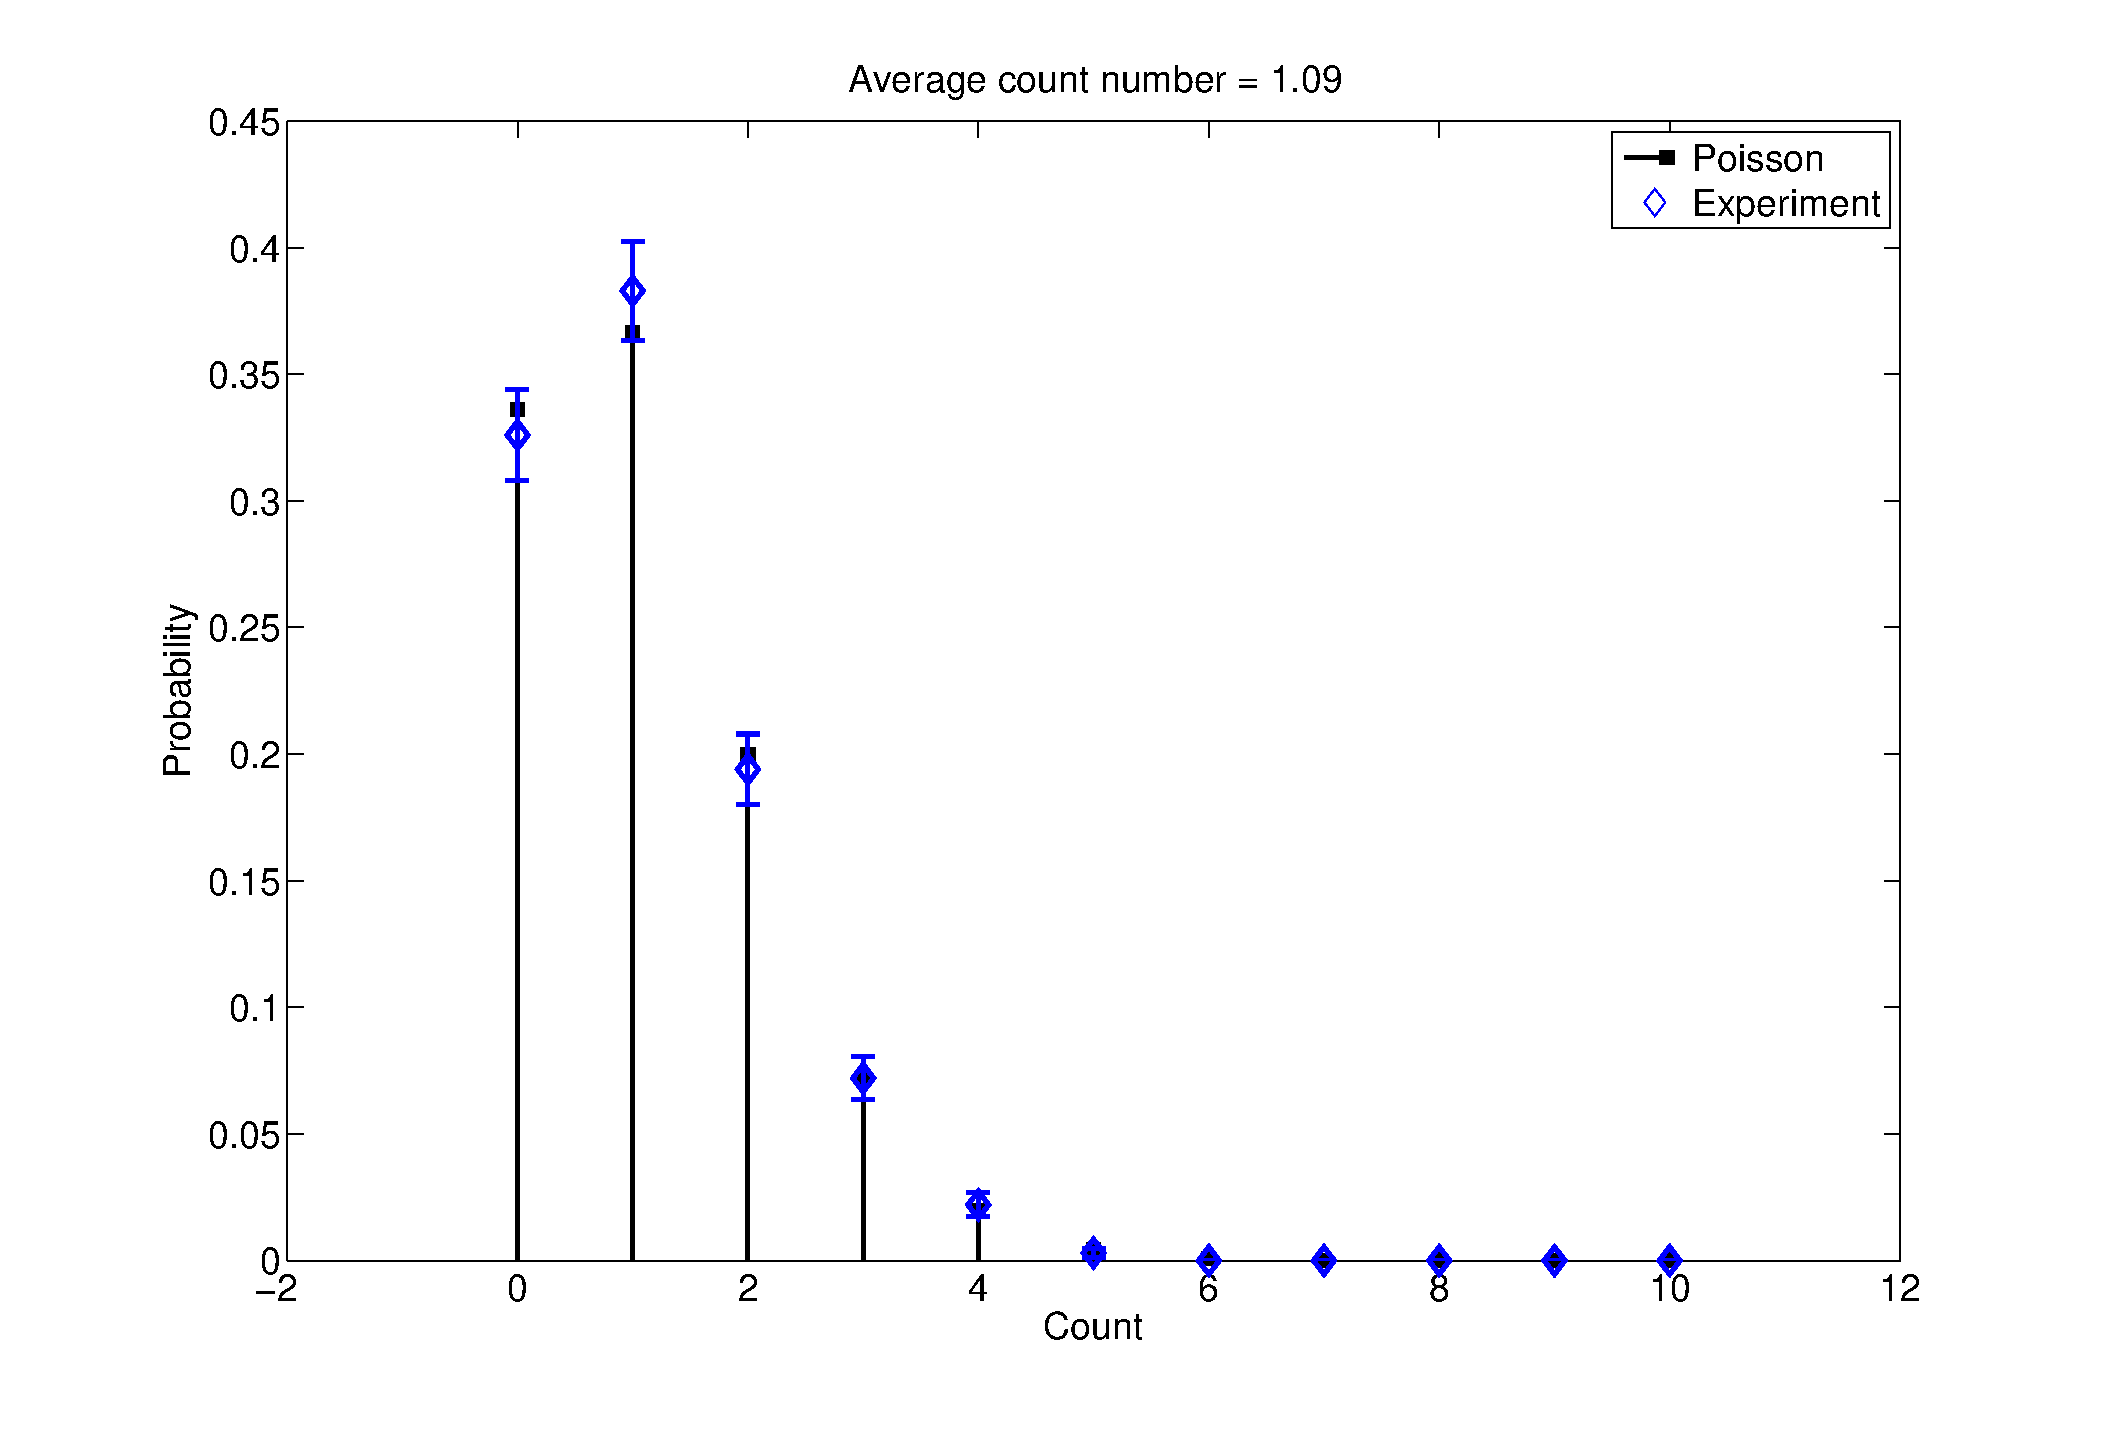
\includegraphics[totalheight=0.6\textwidth]{figs/ci1000}
  \caption{Theoretical and experimental Poisson distribution for constant intensity light with an average photon count = 1.09 photons/ms  and $\chi^{2}$ = 0.254}
  \label{ci1000}
\end{figure}

\begin{figure}[H]
  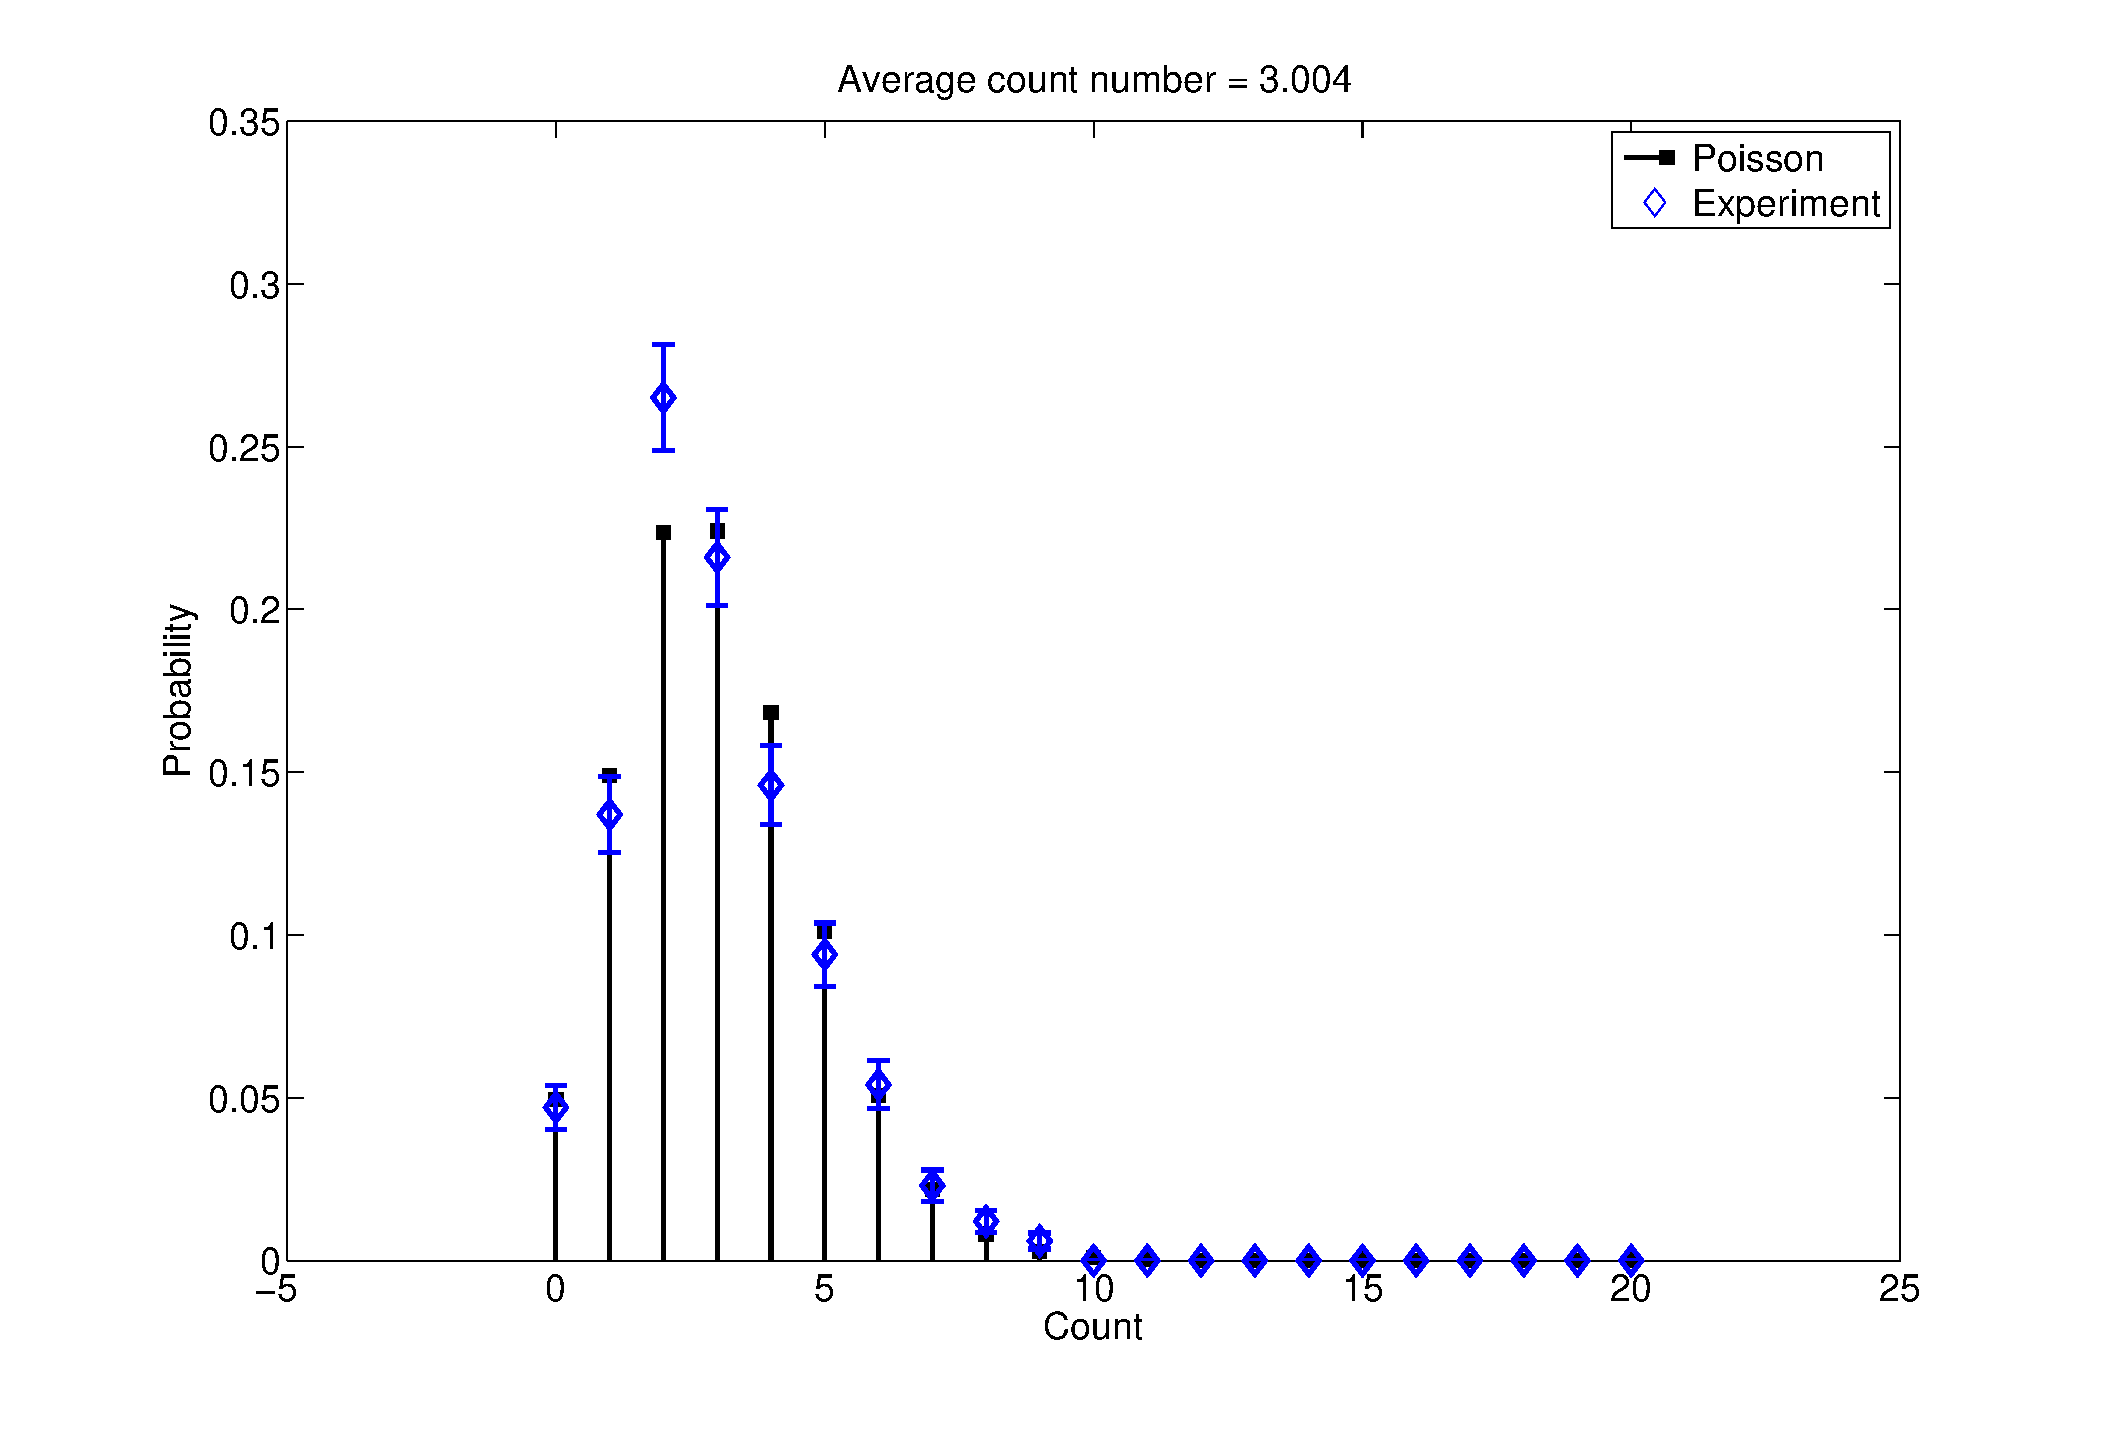
\includegraphics[totalheight=0.6\textwidth]{figs/ci3000}
  \caption{Theoretical and experimental Poisson distribution for constant intensity light with an average photon count = 3.004 photons/ms and $\chi^{2}$ = 0.933}
  \label{ci3000}
\end{figure}

\begin{figure}[H]
  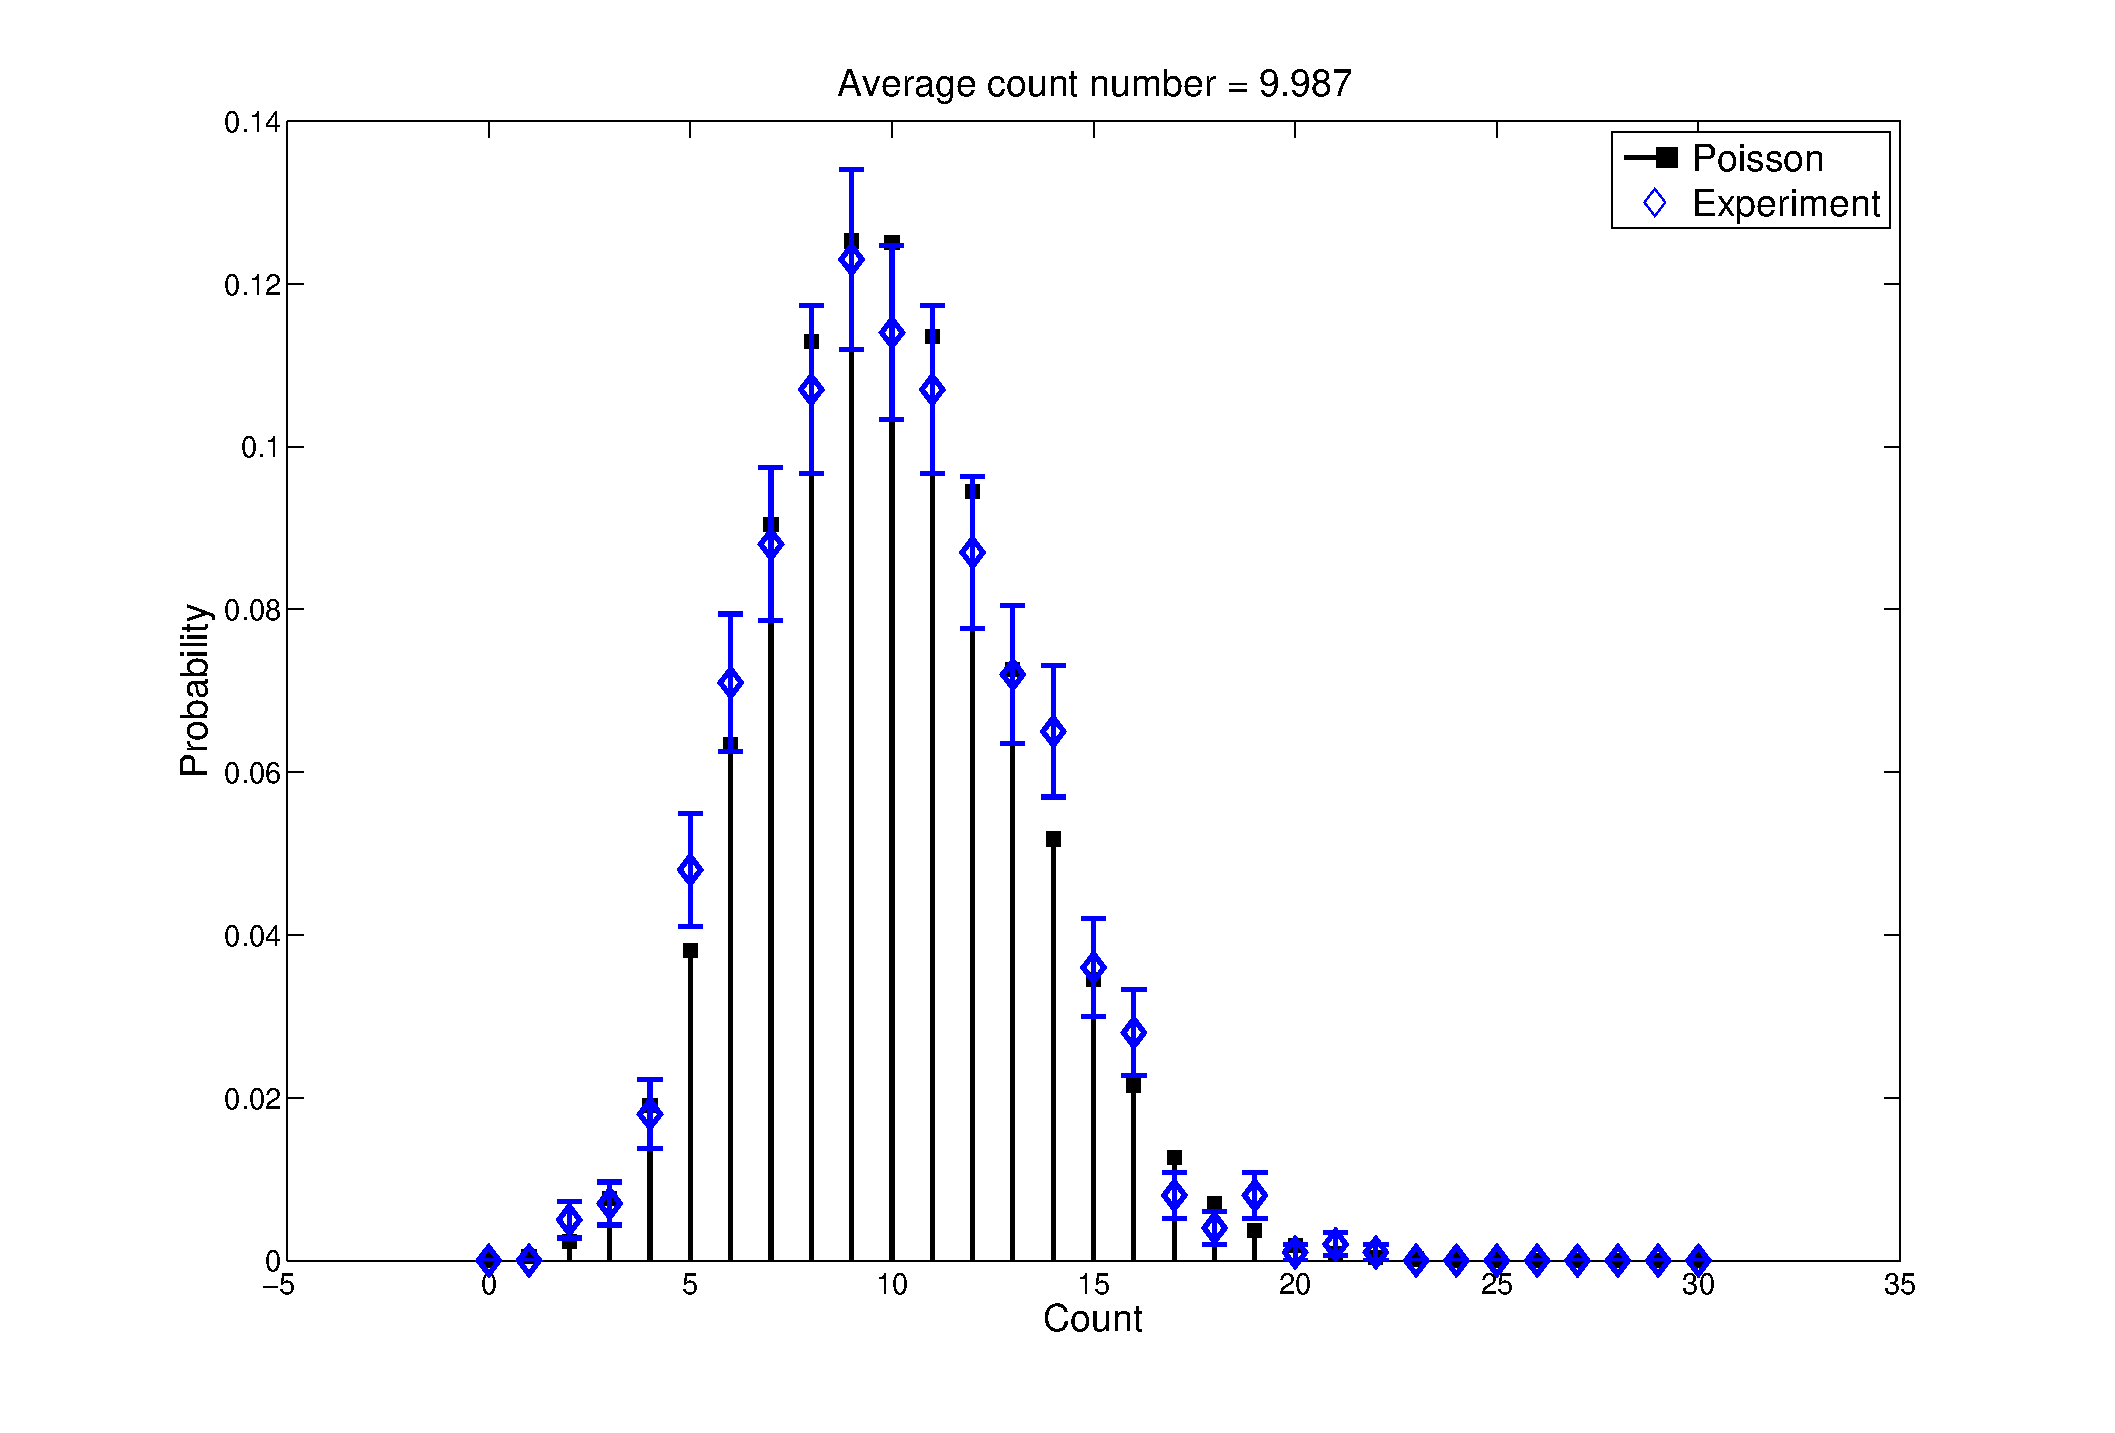
\includegraphics[totalheight=0.6\textwidth]{figs/ci10000}
  \caption{Theoretical and experimental Poisson distribution for constant intensity light with average photon count = 9.987 photons/ms and $\chi^{2}$ = 3.487 and $\chi^{2}$ = 0.843}
  \label{ci10000}
\end{figure}

Figures \ref{pt1000}, \ref{pt3000} and \ref{pt10k} show our probability distributions for randomly scattered light. As shown by the $\chi^{2}$ values and visually our experimental distributions agree with the theoretical Bose-Einstein distribution. One observation that can be made is the probability where 0 events were observed is always lower than predicated. Further, for small counts, just away from 0, the probability is always higher than predicated. We suspect that our resolution for detecting dark may not be fine enough, in which case dark points would be counted as light. Also the HeNe laser that we used is known to emit some blue light in addition to the constant intensity light that we expect, this would also cause dark points to be counted as light. In either or both cases we'd expect to see a sagging at the origin and an uplifting just away from the origin, the exact behavior that our data is exhibiting.

\begin{figure}[H]
  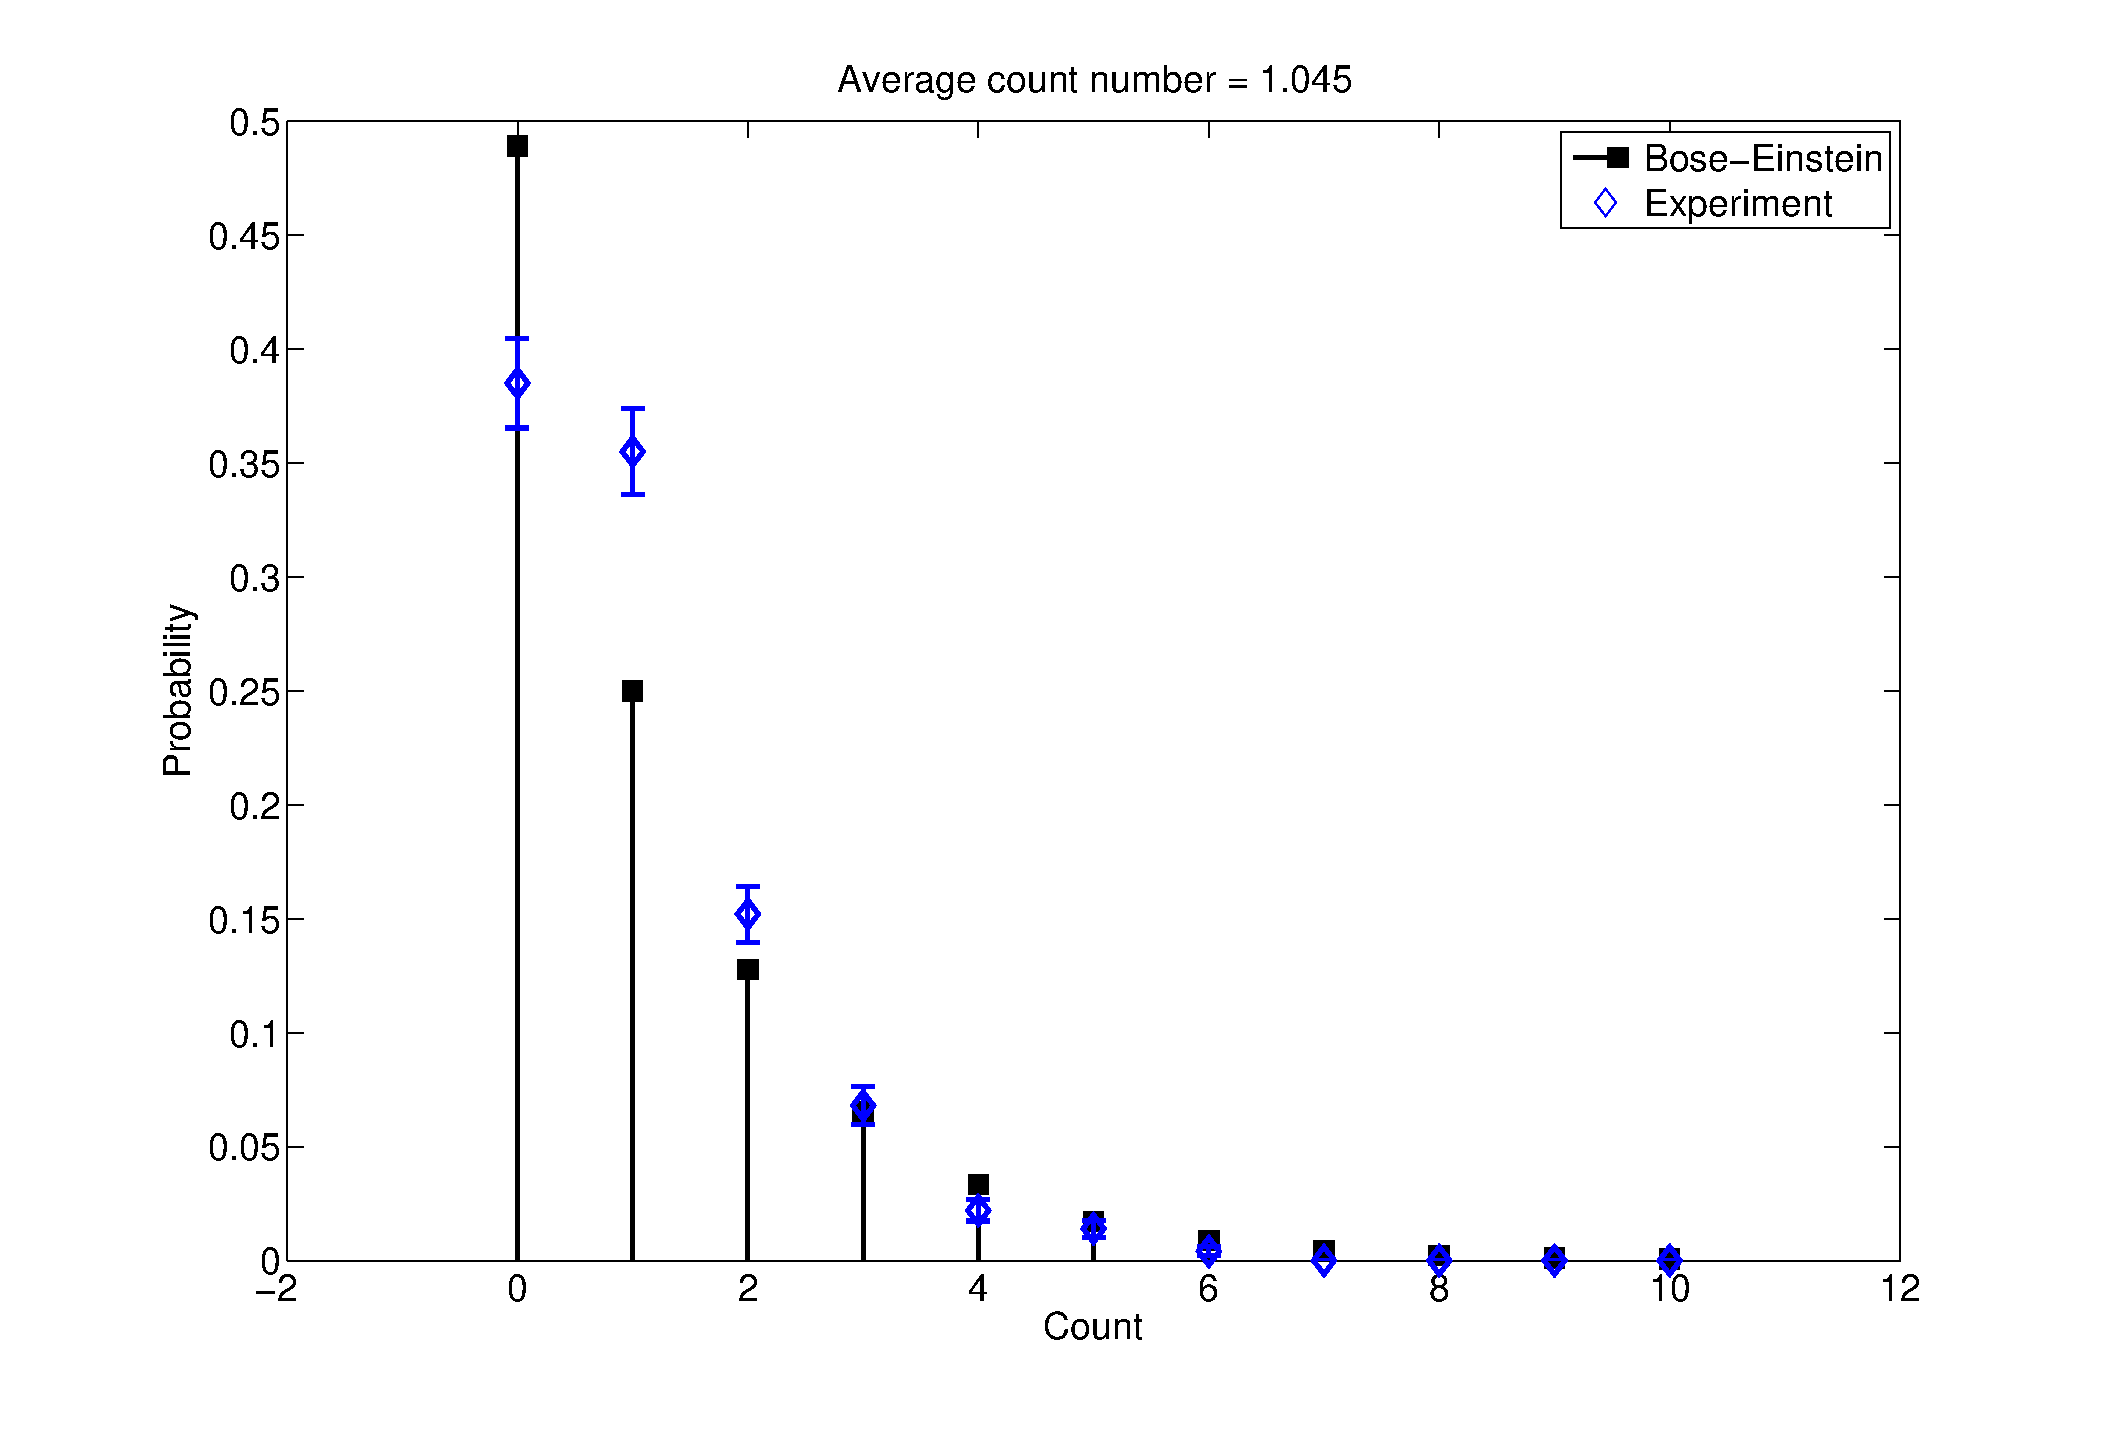
\includegraphics[totalheight=0.6\textwidth]{figs/pt1000}
  \caption{Theoretical and experimental Bose-Einstein distribution for randomly scattered light with average photon count = 1.045 and $\chi^{2}$ = 7.864}
  \label{pt1000}
\end{figure}

\begin{figure}[H]
  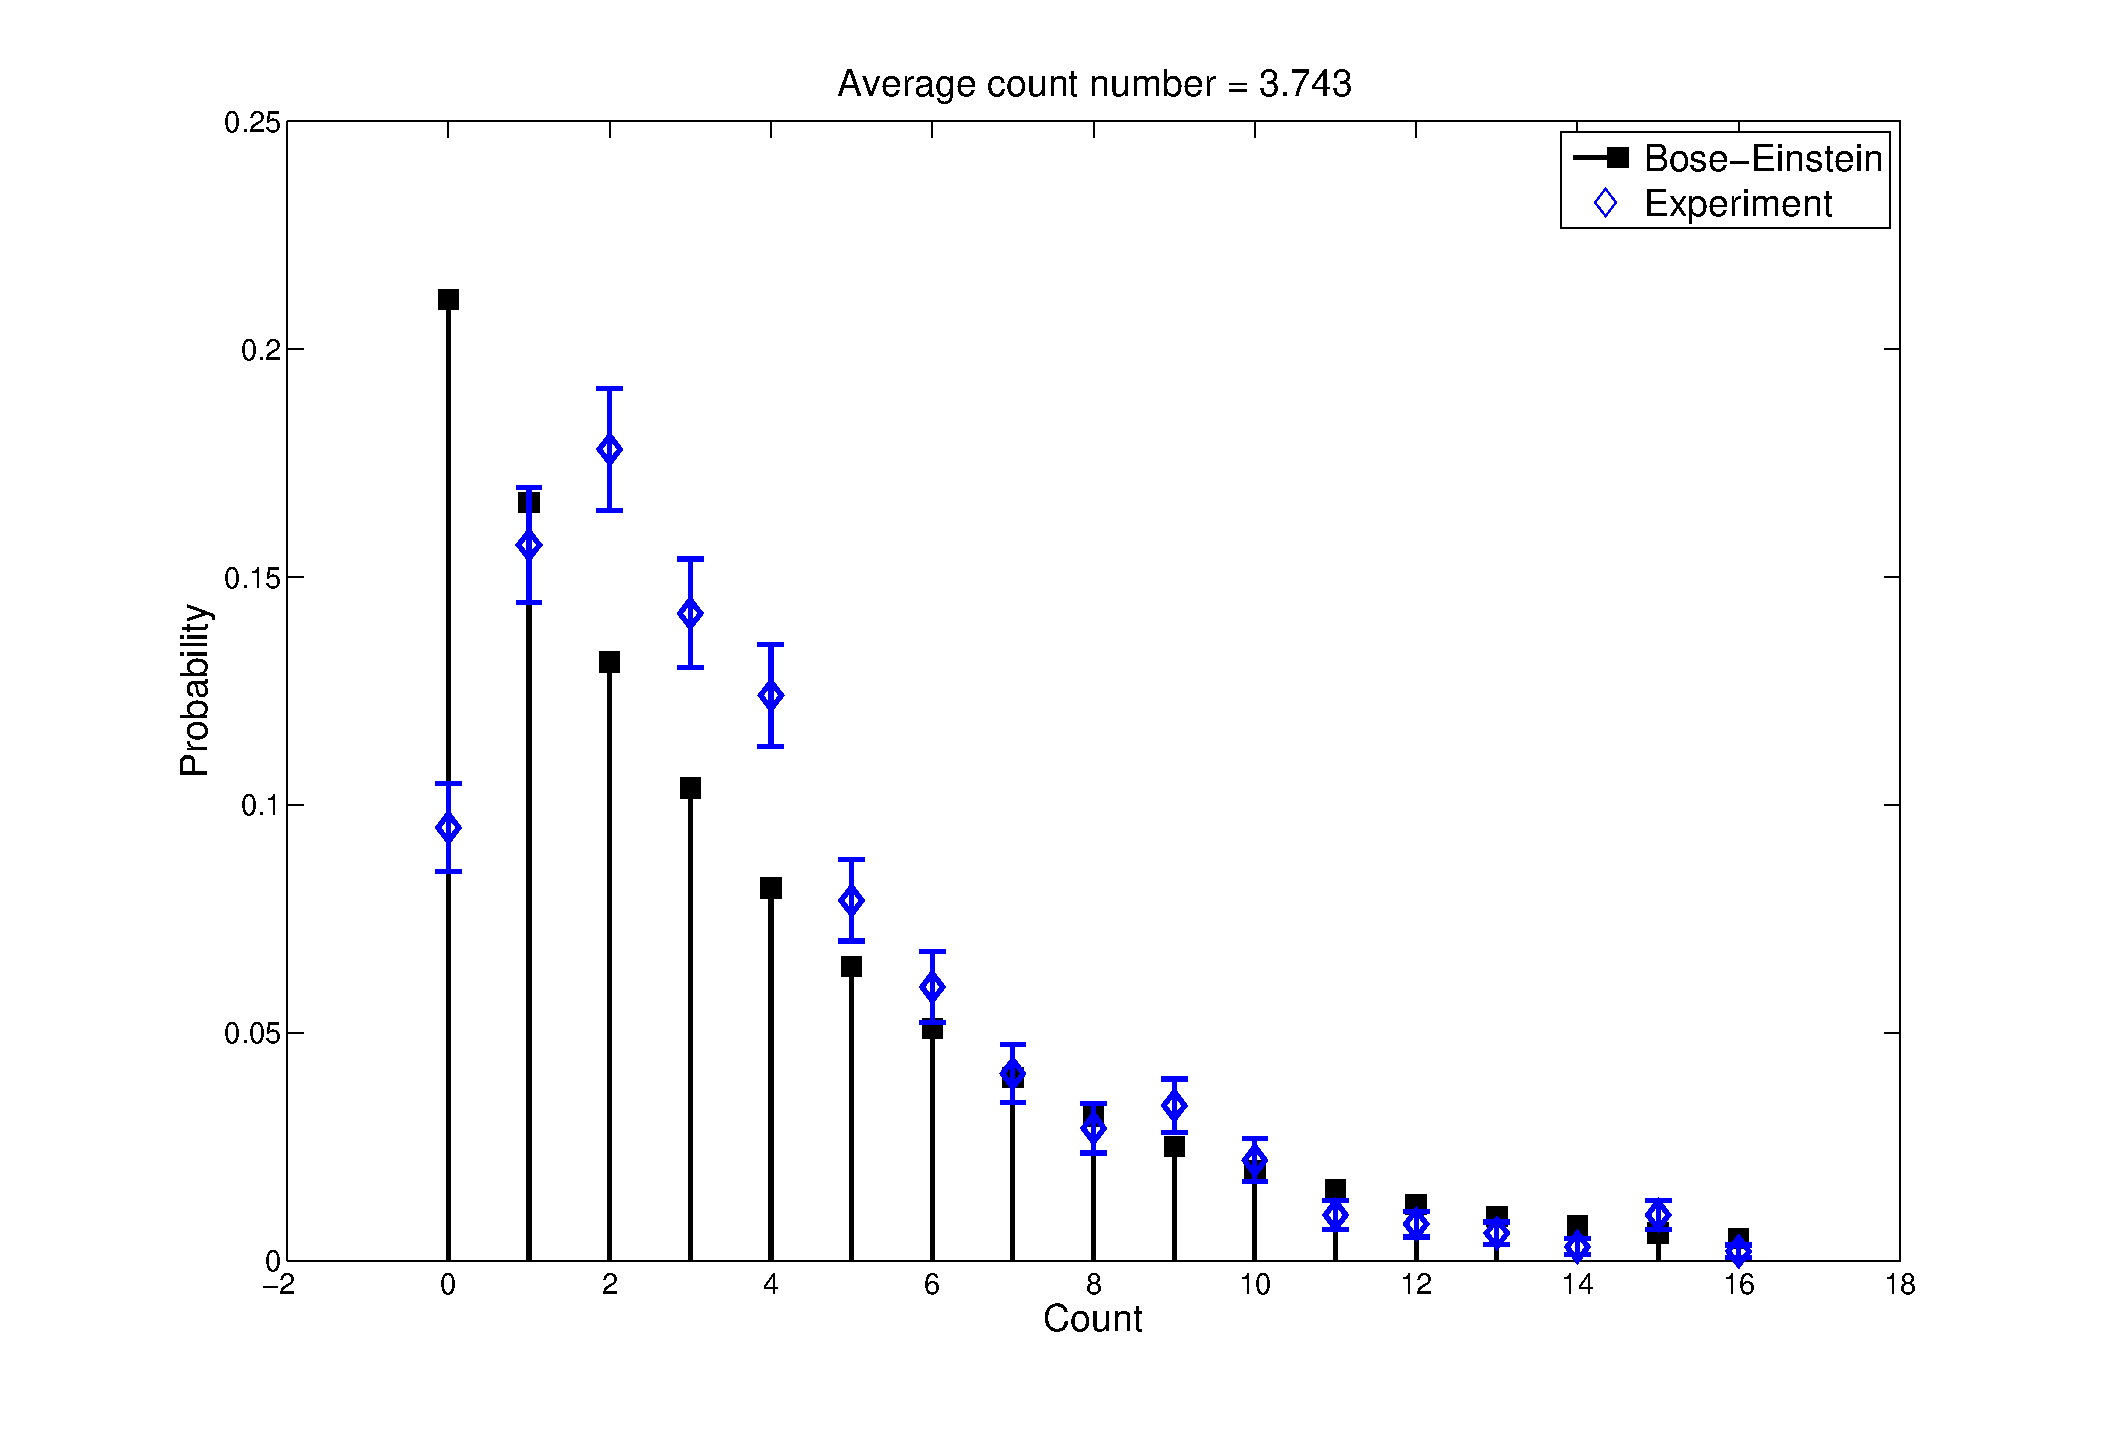
\includegraphics[totalheight=0.6\textwidth]{figs/pt3000}
  \caption{Theoretical and experimental Bose-Einstein distribution for randomly scattered light with average photon count = 3.743 and $\chi^{2}$ = 8.078}
  \label{pt3000}
\end{figure}

\begin{figure}[H]
  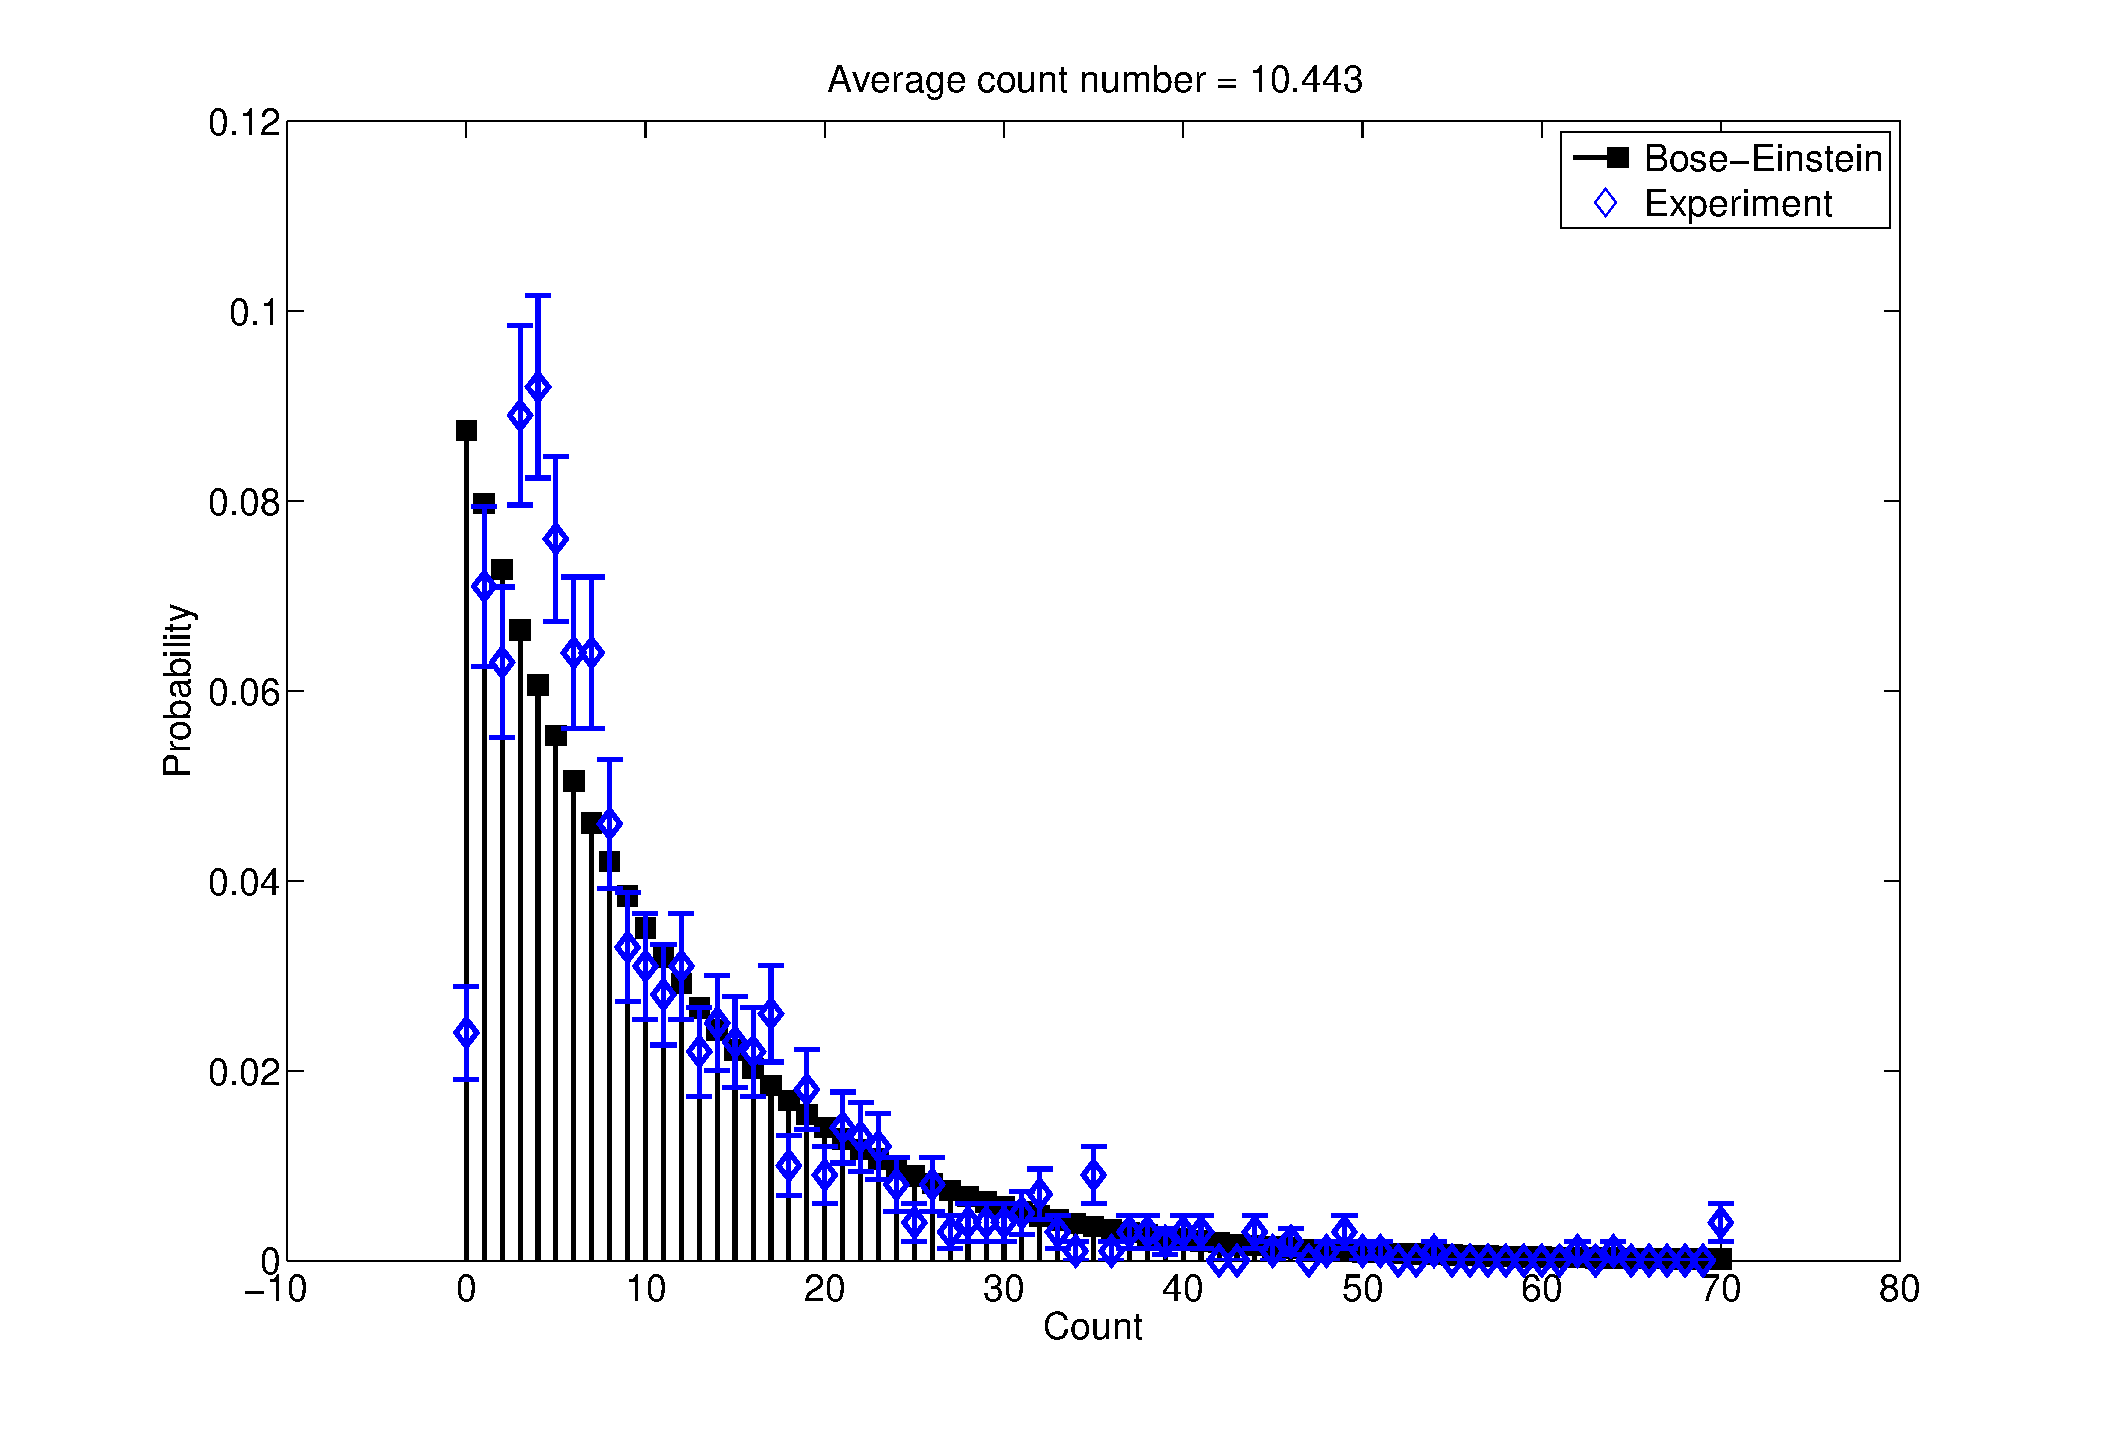
\includegraphics[totalheight=0.6\textwidth]{figs/pt10k}
  \caption{Theoretical and experimental Bose-Einstein distribution for randomly scattered light with average photon count = 10.443 and $\chi^{2}$ = 3.487}
  \label{pt10k}
\end{figure}

\section{Conclusion}
We explored the statistics for photons arriving from a constant intensity and a randomly scattered light source. By constructing probability distributions and calculating $\chi^{2}$ values we found the distribution for constant intensity light to agree with a Poisson distribution and the distribution for randomly scattered light to agree with a Bose-Einstein distribution. We also provided explanation for the slight sagging and uplifting behavior for small counts.



\begin{thebibliography}{99}

\bibitem{manual} Physics Dept., ``Photon Counting and the Statistics of Light'', Quantum Lab, California Polytechnic University, (2013).

\bibitem{koc} P. Koczyk, P. Wiewior, and C. Radzewicz, ``Photon counting statistics-Undergraduate experiment'', Institute of Experimental Physics, Warsaw University, Poland, 1995.

\end{thebibliography}

\end{document}
